\documentclass[handout]{beamer}
\usetheme{metropolis}

% -------------------------------------------------------------------
%   PAQUETES
% -------------------------------------------------------------------
\usepackage[spanish,activeacute]{babel}     % Soporte para español
\usepackage{amsmath, amssymb}              % Matemáticas esenciales
\usepackage{graphicx}                      % Inclusión de imágenes
\usepackage{multirow}                      % Tablas complejas
\usepackage[ruled,vlined,lined]{algorithm2e}% Algoritmos
\usepackage{fontspec}                      % Manejo de fuentes con XeLaTeX
\setsansfont{Lato}                         % Fuente Sans
\setmonofont{Inconsolata}                  % Fuente Monospace
\usepackage{hyperref}                      % Enlaces clicables
\hypersetup{
    colorlinks=true,
    linkcolor=blue,
    urlcolor=magenta
}
\usepackage{dsfont}                        % Símbolos matemáticos adicionales
\usepackage{cases}                         % Entornos para casos matemáticos
\usepackage{epic}                          % Dibujos adicionales
\usepackage{framed,color}                  % Marcos y colores

% -------------------------------------------------------------------
%   INFORMACIÓN DEL DOCUMENTO
% -------------------------------------------------------------------
\title{Procesamiento del Lenguaje Natural \\ \large Word Vectors}
\author[Jorge Ortiz Fuentes]{Jorge Ortiz Fuentes}
\date{\today}

% -------------------------------------------------------------------
%   METADATOS / CONFIGURACIONES
% -------------------------------------------------------------------
\setbeamercolor{normal text}{fg=black,bg=white}
\setbeamercolor{alerted text}{fg=red!80!black}
\setbeamercolor{example text}{fg=green!50!black}
\setbeamertemplate{navigation symbols}{}
\setbeamertemplate{caption}[numbered]
\setbeamertemplate{footline}{
  \begin{beamercolorbox}[wd=\paperwidth,ht=2.5ex,dp=1ex]{frametitle}
    \vspace{1pt}
    \hfill \insertframenumber/\inserttotalframenumber \hspace{3mm}
  \end{beamercolorbox}
}
\metroset{block=fill}
% -------------------------------------------------------------------

\begin{document}

% -------------------------------------------------------------------
%   PORTADA
% -------------------------------------------------------------------
\begin{frame}
  \titlepage
\end{frame}

% -------------------------------------------------------------------
%   ÍNDICE
% -------------------------------------------------------------------
\begin{frame}{Contenido}
  \tableofcontents
\end{frame}

% -------------------------------------------------------------------
%   SECCIÓN: INTRODUCCIÓN A WORD VECTORS
% -------------------------------------------------------------------
\section{Introducción a Word Vectors}

\begin{frame}{Recordatorio: vectores basados en conteo (BoW/TF-IDF)}
  \begin{block}{Limitaciones conocidas}
    \begin{itemize}
      \item Representan palabras/documentos basados en conteos
      \item Generan vectores \textbf{muy largos} (dimensión = |Vocabulario|) y \textbf{dispersos} (muchos ceros)
      \item \textbf{Problema fundamental:} no capturan el \textit{significado} o la \textit{similitud semántica} entre palabras individuales
    \end{itemize}
  \end{block}

  \begin{alertblock}{¿Qué pasa con la similitud coseno?}
    \begin{itemize}
      \item La similitud coseno entre vectores BoW/TF-IDF mide el solapamiento de términos, no necesariamente la similitud semántica intrínseca.
    \end{itemize}
  \end{alertblock}
\end{frame}

\begin{frame}{Word Vectors: una alternativa a la dispersión} 
  \begin{block}{¿Qué son los word vectors?} 
    Son una forma de representar palabras como vectores
    \begin{itemize} \item El objetivo principal es capturar el \textbf{significado} de las palabras y las \textbf{relaciones semánticas} entre ellas. 
      \item Pueden ser \textbf{densos} (pocos o ningún cero) o \textbf{dispersos}, dependiendo del método de creación. Los vectores \textbf{densos (embeddings)} son el enfoque predominante. 
      \item Se aprenden automáticamente a partir de grandes cantidades de texto (corpus) mediante técnicas que modelan el contexto de las palabras. 
    \end{itemize} 
  \end{block} 
\end{frame}

\begin{frame}{Hacia un espacio vectorial semántico}
  \begin{itemize}
  \item \textbf{Idea clave:} La posición de una palabra en este nuevo espacio vectorial \textit{codifica} sus propiedades semánticas y sintácticas.
   \item Palabras con significados similares tendrán vectores cercanos en este espacio.
   \item Por ejemplo, la \textbf{similitud coseno} entre los vectores de \textit{rey} y \textit{reina} será alta, reflejando su relación semántica.
   \item Estos vectores son fundamentales en las arquitecturas modernas de NLP basadas en redes neuronales.
 \end{itemize}
\end{frame}

% -------------------------------------------------------------------
%   SECCIÓN: VECTORES DISTRIBUCIONALES
% -------------------------------------------------------------------
\section{Vectores distribucionales}

\begin{frame}{¿Cómo definimos `perro'?}
  \begin{center}
    \includegraphics[width=0.6\textwidth]{pics/perro1.png}
    \vspace{0.5cm}
  \end{center}
\end{frame}

\begin{frame}{El desafío de definir ‘por lo que es’}
  \setkeys{Gin}{width=0.7\textwidth, keepaspectratio}
  \begin{columns}[T,totalwidth=\textwidth]
    \begin{column}{0.48\textwidth}
      \centering
      \includegraphics{pics/perro2.png}\par\vspace{0.2cm}
      \includegraphics{pics/perro3.png}
    \end{column}
    \begin{column}{0.48\textwidth}
      \centering
      \includegraphics{pics/perro4.png}\par\vspace{0.2cm}
      \includegraphics{pics/perro5.png}
    \end{column}
  \end{columns}
  \vspace{0.5cm}
\end{frame}

\begin{frame}{¿Cómo asignamos significado?}
  \begin{block}{La idea Saussureana: significado por oposición}
    \begin{itemize}
      \item Ferdinand de Saussure, lingüista suizo, propuso que el significado no es inherente a los signos, sino que surge de su relación con otras signos dentro de un sistema
      \item \textbf{Valor negativo}: el significado se define por lo que \textit{no} es
      \item Ejemplo: ¿Qué es un `perro'? Solo podemos definirlo en contraste con otros conceptos (no es un gato, no es un lobo, no es un mueble, etc.)
      \item El significado es relacional y diferencial, no una propiedad positiva intrínseca
    \end{itemize}
  \end{block}
\end{frame}

\begin{frame}{Hipótesis distribucional}
  \begin{columns}
    \begin{column}{\textwidth}
      \begin{block}{Principio fundamental}
        \begin{itemize}
          \item \textbf{Hipótesis Distribucional} \cite{harris1954}: palabras que aparecen en los mismos \textbf{contextos} tienden a tener significados similares.
          \item ``Una palabra se caracteriza por la \textbf{compañía} que mantiene'' \cite{firth1957}.
          \item ``El significado de una palabra es su \textbf{uso} en el lenguaje'' \cite{wittgenstein1953}.
        \end{itemize}
      \end{block}
    \end{column}
  \end{columns}
\end{frame}

\begin{frame}{Representaciones distribucionales}
 \begin{columns}
  \begin{column}{0.6\textwidth}
    \begin{alertblock}{Idea central}
      \begin{itemize}
        \item Basado en la hipótesis distribucional, podemos representar palabras mediante vectores que capturen sus contextos típicos
      \item Estos vectores se denominan \textbf{representaciones distribucionales}
      \item La idea es que la similitud entre estos vectores refleje la similitud semántica entre las palabras
    \end{itemize}
  \end{alertblock}
  % El bloque "Construcción" se movió a la siguiente diapositiva
  \end{column}
  \begin{column}{0.4\textwidth}
    \begin{center}
      \includegraphics[width=0.9\textwidth]{pics/distributional_hypothesis.png}
    \end{center}
  \end{column}
 \end{columns}
\end{frame}

\begin{frame}{Matrices palabra-contexto: conceptos básicos}
  \begin{block}{Construcción}
    Una forma posible es usar \textbf{vectores de alta dimensionalidad} donde cada dimensión corresponde a alguna medida de asociación con un contexto específico (ej. otra palabra, un documento).
  \end{block}
  \begin{itemize}
    \item Una forma de construir vectores distribucionales es mediante las matrices palabra-contexto $M$
    \item Cada celda $(i,j)$ representa la asociación entre una \textbf{palabra objetivo} $w_i$ y un \textbf{contexto} $c_j$ obtenido de un corpus
    \item Los contextos se definen comúnmente como ventanas de palabras que rodean a $w_i$
  \end{itemize}
\end{frame}

\begin{frame}{Matrices palabra-contexto: parámetros y observaciones}
  \begin{block}{Parámetros importantes}
    \begin{itemize}
      \item La longitud de la ventana $k$ (entre 1 y 8 palabras a ambos lados de $w_i$)
      \item Si el vocabulario de palabras objetivo y de contexto es el mismo, $M$ tiene dimensionalidad $|\mathcal{V}| \times |\mathcal{V}|$
    \end{itemize}
  \end{block}
  
  \begin{alertblock}{Observación clave}
    \pause
    \small
    Ventanas más cortas capturan información \textbf{sintáctica} (por ejemplo, POS), mientras que ventanas más largas capturan similitud \textbf{semántica}.
  \end{alertblock}
\end{frame}

\begin{frame}{Ejemplo de vectores distribucionales con ventanas de contexto de tamaño 1}
  \begin{block}{Ejemplo ilustrativo}
    A continuación, presentamos un ejemplo con las siguientes oraciones:
    \begin{itemize}
      \item I like deep learning
      \item I like NLP
      \item I enjoy flying
    \end{itemize}
    Este ejemplo ilustra cómo se construyen vectores distribucionales usando ventanas de contexto de tamaño 1, donde cada dimensión representa la frecuencia de co-ocurrencia con otra palabra del vocabulario
  \end{block}
\end{frame}

\begin{frame}{Ejemplo de vectores distribucionales con ventanas de contexto de tamaño 1}
  \begin{center}
    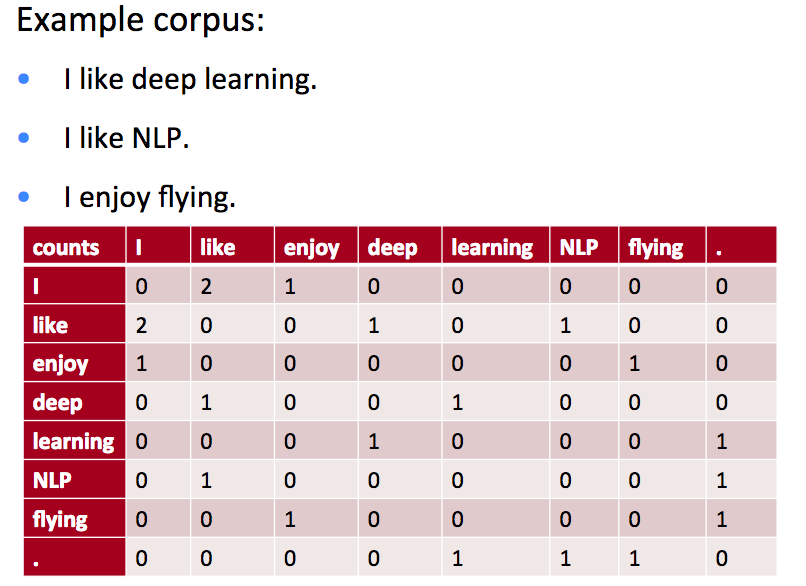
\includegraphics[scale=0.28]{pics/distributionalSocher.png}
    
    \vspace{0.3cm}
    \footnotesize{Ejemplo tomado de: \url{http://cs224d.stanford.edu/lectures/CS224d-Lecture2.pdf}}
  \end{center}
\end{frame}


% -------------------------------------------------------------------
%   SECCIÓN: VECTORES DISTRIBUIDOS (WORD EMBEDDINGS)
% -------------------------------------------------------------------
\section{Vectores distribuidos (word embeddings)}

\begin{frame}{Word embeddings}
  \begin{block}{Limitaciones de los métodos basados en conteo}
    \begin{itemize}
      \item Los vectores distribucionales basados en conteo aumentan en tamaño con el vocabulario
      \item Almacenar explícitamente la matriz de co-ocurrencia puede consumir mucha memoria
      \item Algunos modelos de clasificación no escalan bien a datos de alta dimensionalidad
    \end{itemize}
  \end{block}
  
  \begin{alertblock}{Solución: word embeddings}
    \begin{itemize}
      \item La comunidad de redes neuronales prefiere usar \textbf{representaciones distribuidas} o \textbf{word embeddings}
      \item Son vectores densos de palabras de baja dimensionalidad entrenados con redes neuronales
    \end{itemize}
  \end{alertblock}
\end{frame}

\begin{frame}{Características de los word embeddings}
  \begin{block}{Propiedades clave}
    \begin{itemize}
      \item Las dimensiones no son directamente interpretables, representan características latentes de la palabra
      \item Capturan propiedades sintácticas y semánticas útiles
      \item Se han convertido en un componente crucial de las arquitecturas de redes neuronales para NLP
    \end{itemize}
  \end{block}
  
  \begin{alertblock}{Nota importante}
    La idea fundamental: El significado de la palabra está distribuido sobre una combinación de dimensiones.
  \end{alertblock}
\end{frame}

\begin{frame}{Enfoques para obtener word embeddings}
  \begin{block}{Dos enfoques principales}
    \begin{enumerate}
      \item \textbf{Capas de embedding}: usar una capa de embedding en una arquitectura de red neuronal específica para una tarea, entrenada con ejemplos etiquetados (ej. análisis de sentimiento).
      
      \item \textbf{Word embeddings pre-entrenados}: crear una tarea predictiva auxiliar a partir de corpus no etiquetados (ej. predecir la siguiente palabra) en la que los word embeddings surgirán naturalmente de la arquitectura de la red neuronal.
    \end{enumerate}
  \end{block}
  
  \begin{alertblock}{Estrategia combinada}
    Inicializa la capa de embedding con embeddings pre-entrenados para aprovechar lo mejor del aprendizaje supervisado y no supervisado.
  \end{alertblock}
\end{frame}

\begin{frame}{Modelos Populares de Word Embeddings}
  \begin{block}{Modelos más utilizados}
    \begin{itemize}
      \item \textbf{Word2Vec:} Utiliza las arquitecturas CBOW y Skip-Gram para aprender embeddings a partir de grandes corpus, capturando relaciones semánticas y sintácticas \cite{Mikolov2013}.
      \item \textbf{GloVe:} (Global Vectors) Se basa en estadísticas globales de co-ocurrencia para generar representaciones vectoriales que reflejan similitudes semánticas \cite{penningtonSM14}.
      \item \textbf{FastText:} Extiende Word2Vec incorporando información de subpalabras, lo que mejora la representación de palabras poco frecuentes y morfológicamente complejas \cite{bojanowski2016enriching}.  
    \end{itemize}
  \end{block}

\end{frame}

% -------------------------------------------------------------------
%   SECCIÓN: WORD2VEC
% -------------------------------------------------------------------
\section{Word2Vec}

\begin{frame}{Word2Vec: Introducción}
  \begin{block}{¿Qué es Word2Vec?}
    \begin{itemize}
      \item Word2Vec es un paquete de software que implementa dos arquitecturas de redes neuronales para entrenar word embeddings.
      \item Fue introducido por Tomas Mikolov y colaboradores en Google (2013).
      \item Permite aprender representaciones vectoriales densas de palabras a partir de grandes corpus de texto.
    \end{itemize}
  \end{block}
\end{frame}

\begin{frame}{Arquitecturas de Word2Vec}
  \begin{block}{Principales enfoques}
    \begin{itemize}
      \item \textbf{Modelo Skip-gram:} Dada una palabra central, se predicen las palabras de su contexto.
      \item \textbf{Modelo Continuous Bag-of-Words (CBOW):} A partir de las palabras del contexto, se predice la palabra central.
    \end{itemize}
  \end{block}
\end{frame}


\begin{frame}{Modelo Skip-gram: Conceptos básicos}
  \begin{block}{Funcionamiento general}
    \begin{itemize}
      \item Para cada posición $t$, toma la palabra central $w_t$.
      \item Para cada palabra de contexto $c$ en la ventana $c_{1:k}$, entrena un clasificador independiente que comparte pesos.
      \item La capa de entrada es un vector one-hot de dimensión $|V|$; la capa oculta (proyección) es de dimensión $d$.
      \item No se concatenan los $k$ vectores antes de la salida; cada par $(w_t,c)$ produce su propia loss.
    \end{itemize}
  \end{block}
  \begin{alertblock}{Representación inicial}
    Vectores one-hot en la entrada y en la salida antes de proyectar a $d$ dimensiones.
  \end{alertblock}
\end{frame}

\begin{frame}{Arquitectura del Modelo Skip-gram}
  \begin{columns}
    \begin{column}{0.5\textwidth}
      \begin{block}{Estructura de la red}
        \begin{itemize}
          \item Compartición de pesos entre las $k$ predicciones de contexto.
          \item Capa oculta de tamaño $d$ (hiperparámetro, normalmente $d \ll |V|$).
        \end{itemize}
      \end{block}
    \end{column}
    \begin{column}{0.5\textwidth}
      \centering
      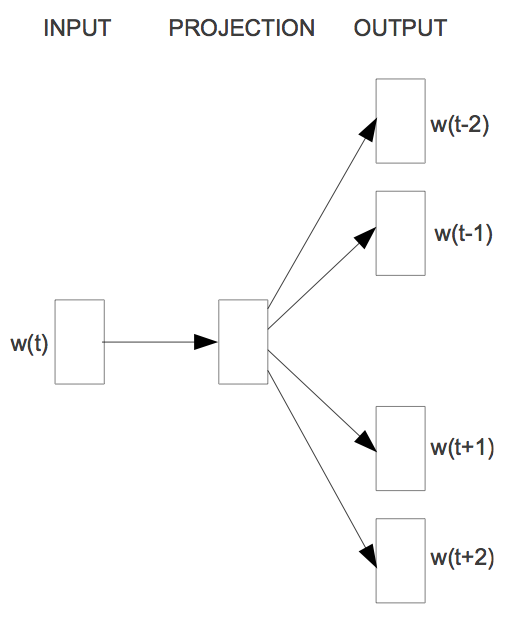
\includegraphics[scale=0.5]{pics/skip-gram.png}
    \end{column}
  \end{columns}
\end{frame}

\begin{frame}{Objetivo del modelo Skip-gram}
  \begin{block}{Meta principal}
    \begin{itemize}
      \item Aprender vectores $\vec{w}$ y $\vec{c}$ tales que cada palabra central prediga bien su contexto real.
      \item Maximizar la probabilidad conjunta de observar todos los pares $(w_t,c)$ en el corpus $D$:
      \[
        \sum_{(w,c) \in D} \log P(c\mid w)
      \]
    \end{itemize}
  \end{block}
\end{frame}

\begin{frame}{Cálculo de $P(c\mid w)$: la función softmax}
  \begin{block}{Definición}
    La probabilidad de observar una palabra de contexto $c$ dada una palabra central $w$ se calcula usando la función softmax:
    \[P(c\mid w)=\frac{e^{\vec{c}\cdot\vec{w}}}{\sum_{c'\in V} e^{\vec{c}'\cdot\vec{w}}}\]
    \begin{itemize}
        \item $\sum_{c'\in V}$: normalización sobre todo el vocabulario $V$ para obtener una distribución de probabilidad
    \end{itemize}
  \end{block}
  \begin{alertblock}{Desafío computacional}
    Calcular el denominador requiere considerar \textit{todas} las palabras del vocabulario $V$, lo cual es computacionalmente muy costoso si $|V|$ es grande (cientos de miles o millones).
  \end{alertblock}
\end{frame}

\begin{frame}{Optimizaciones para el cálculo de $P(c\mid w)$}
  \begin{block}{Alternativas eficientes al softmax completo}
    El cálculo del denominador en la función softmax es computacionalmente prohibitivo para vocabularios grandes. Se pueden ocupar técnicas de optimización para hacerlo más eficiente:
    \begin{itemize}
        \item Negative sampling
        \item Hierarchical softmax
    \end{itemize}
    Estas técnicas aproximan la normalización completa o reducen la carga computacional de otras maneras.
  \end{block}
\end{frame}

\begin{frame}{Optimización: negative sampling}
  \begin{block}{Idea principal}
    Transforma el problema multiclase (predecir la palabra de contexto correcta entre $|V|$ opciones) en un conjunto de problemas de clasificación binaria.
    \begin{itemize}
        \item Para cada par real $(w, c)$, se considera una muestra positiva
        \item Se generan $n$ muestras "negativas" $(w, c')$
        \item Se entrena un clasificador logístico (usando la función sigmoide) para distinguir entre la muestra positiva y las negativas
        \item El número de muestras negativas $n$ es un hiperparámetro (usualmente 5-20)
    \end{itemize}
    Evita la costosa suma sobre todo el vocabulario $V$.
  \end{block}
\end{frame}

\begin{frame}{Optimización: hierarchical softmax}
  \begin{block}{Estructura y funcionamiento}
    Utiliza un árbol binario para representar el vocabulario.
    \begin{itemize}
        \item Cada hoja del árbol corresponde a una palabra del vocabulario $V$
        \item Para calcular $P(c|w)$, se navega desde la raíz hasta la hoja correspondiente a $c$
        \item En cada nodo interno del camino, se toma una decisión binaria (izquierda o derecha) usando una función sigmoide y un vector asociado al nodo
        \item La probabilidad final $P(c|w)$ es el producto de las probabilidades sigmoides a lo largo del camino
    \end{itemize}
    Reduce la complejidad computacional de $O(|V|)$ a $O(\log |V|)$.
  \end{block}
\end{frame}

\begin{frame}{Skip-gram: Resumen y buenas prácticas}
  \begin{itemize}
    \item Cada contexto se predice con un clasificador separado que comparte parámetros.
    \item Negative Sampling y Hierarchical Softmax hacen viable el entrenamiento en vocabularios grandes.
    \item Ajustar hiperparámetros clave:
      \begin{itemize}
        \item Dimensión $d$ de embeddings
        \item Tamaño de ventana $k$
        \item Número de negativos $n$
        \item Tasa de subsampling para palabras frecuentes
      \end{itemize}
  \end{itemize}
\end{frame}

\begin{frame}{Continuous Bag of Words (CBOW)}
  \begin{columns}
    \begin{column}{0.5\textwidth}
      \begin{block}{Enfoque alternativo}
        \begin{itemize}
          \item Similar al modelo skip-gram pero ahora la palabra central se predice a partir del contexto circundante
          \item Invierte la dirección de predicción respecto al Skip-gram
        \end{itemize}
      \end{block}
    \end{column}
    
    \begin{column}{0.5\textwidth}
      \begin{center}
        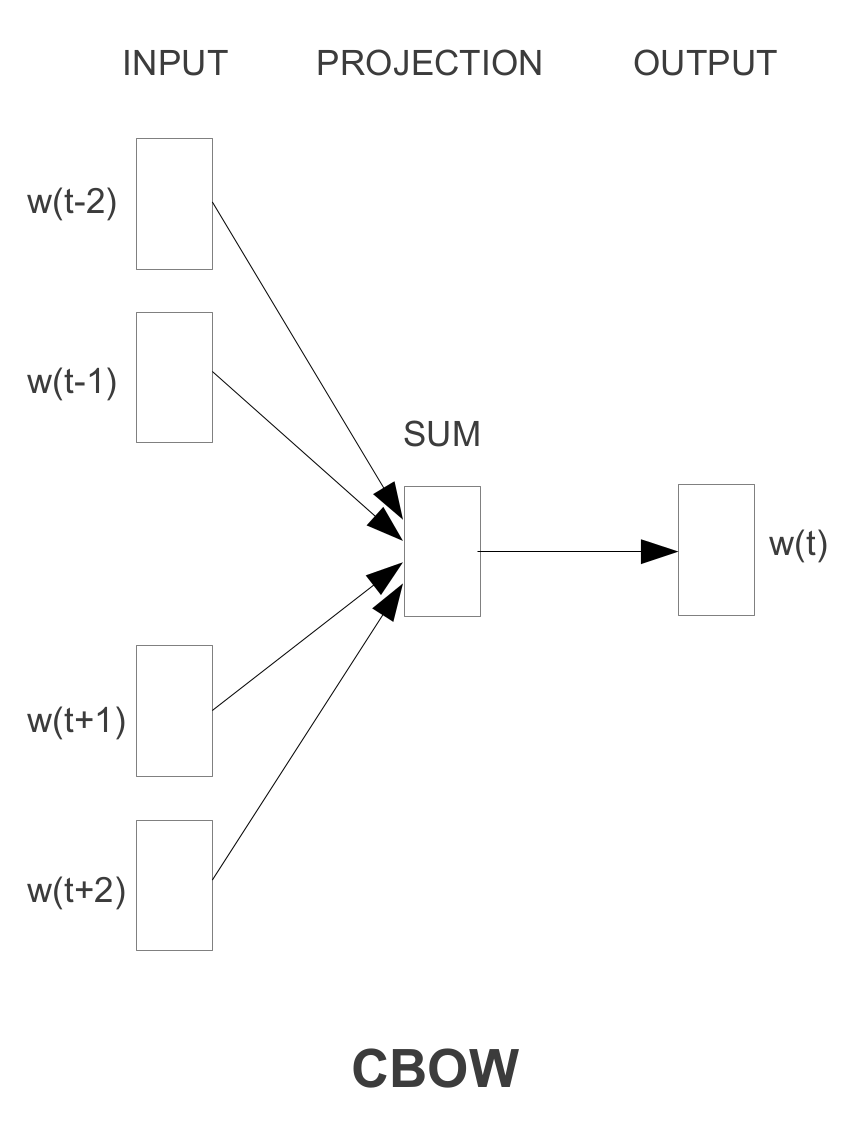
\includegraphics[scale=0.70]{pics/CBOW.png}
      \end{center}
    \end{column}
  \end{columns}
\end{frame}

\begin{frame}{CBOW vs Skip-gram: ¿Cuándo usar cuál?}
  \begin{columns}[T] % Alineación superior para los bloques
    \begin{column}{0.48\textwidth}
      \begin{block}{CBOW}
        \begin{itemize}
          \item Predice la palabra central desde el contexto
          \item Más rápido de entrenar
          \item Mejor para palabras frecuentes
        \end{itemize}
      \end{block}
    \end{column}
    \begin{column}{0.48\textwidth}
      \begin{block}{Skip-gram}
        \begin{itemize}
          \item Predice el contexto desde la palabra central
          \item Más lento pero mejor con palabras raras
          \item Funciona bien con corpus pequeños
        \end{itemize}
      \end{block}
    \end{column}
  \end{columns}
  \begin{alertblock}{Recomendación general}
    Skip-gram suele funcionar mejor para la mayoría de las tareas, especialmente si el corpus no es masivo. CBOW es una alternativa más rápida si la velocidad es crítica.
  \end{alertblock}
\end{frame}

% -------------------------------------------------------------------
%   SECCIÓN: GLOVE
% -------------------------------------------------------------------
\section{GloVe}

\begin{frame}{GloVe: vectores globales para palabras}
  \begin{block}{Idea central}
    \begin{itemize}
      \item GloVe crea una matriz de co-ocurrencias global para todo el corpus.
      \item Captura relaciones semánticas aprovechando estadísticas globales.
    \end{itemize}
  \end{block}
  \begin{alertblock}{Enfoque híbrido}
    \begin{itemize}
      \item Combina conteos globales (count-based) y aprendizaje predictivo.
      \item Usa una función de ponderación para suavizar el efecto de conteos extremos.
      \item A diferencia de Word2Vec, mira todo el corpus en lugar de sólo ventanas locales.
    \end{itemize}
  \end{alertblock}
\end{frame}

\section{FastText}

\begin{frame}{FastText: vectores enriquecidos con subpalabras}
  \begin{block}{Idea central}
    \begin{itemize}
      \item Extensión de Word2Vec que representa cada palabra como la suma de vectores de sus n-gramas.
      \item Entrena de forma muy eficiente usando skip-gram o CBOW con negative sampling.
    \end{itemize}
  \end{block}
  \begin{alertblock}{Enfoque}
    \begin{itemize}
      \item Descompone cada palabra en sub-componentes.
      \item Aprende vectores para cada n-grama y luego los agrupa para formar el embedding de la palabra.
      \item Captura información morfológica y mejora la calidad de embeddings para palabras raras o desconocidas.
    \end{itemize}
  \end{alertblock}
\end{frame}


\begin{frame}{FastText vs Word2Vec y GloVe}
  \begin{columns}[T]
      \begin{column}{0.48\textwidth}
          \begin{block}{Fortalezas de FastText}
              \begin{itemize}
                  \item Capacidad para generar vectores para palabras desconocidas
                  \item Buen rendimiento en lenguas morfológicamente ricas
              \end{itemize}
          \end{block}
      \end{column}
      \begin{column}{0.48\textwidth}
          \begin{block}{Consideraciones}
              \begin{itemize}
                  \item Modelos más grandes (almacena vectores para n-gramas)
                  \item Entrenamiento potencialmente más lento que Word2Vec
                  \item La calidad puede depender de la elección de n-gramas
              \end{itemize}
          \end{block}
      \end{column}
  \end{columns}
\end{frame}

% -------------------------------------------------------------------
%   SECCIÓN: ANALOGÍAS Y EVALUACIÓN
% -------------------------------------------------------------------
\section{Analogías y evaluación}

\begin{frame}{Analogías de palabras: relaciones semánticas}
  \begin{block}{Relaciones semánticas}
    \begin{itemize}
      \item Los word embeddings pueden capturar ciertas relaciones semánticas, por ejemplo, relaciones masculino-femenino, tiempo verbal y país-capital entre palabras
      \item Por ejemplo, se encuentra la siguiente relación para word embeddings entrenados con Word2Vec: $\vec{w}_{king} - \vec{w}_{man} + \vec{w}_{woman} \approx \vec{w}_{queen}$
    \end{itemize}
  \end{block}
\end{frame}

\begin{frame}{Analogías de palabras: ejemplo visual}
  \begin{center}
    
\includegraphics[width=1\textwidth]{pics/linear-relationships.png}
    \vspace{0.5cm}
    \footnotesize{Fuente: \url{https://www.tensorflow.org/tutorials/word2vec}}
  \end{center}
\end{frame}

\begin{frame}{Evaluación de word embeddings}
  \begin{block}{Métodos de evaluación}
    \begin{itemize}
      \item Existen muchos conjuntos de datos con asociaciones de pares de palabras anotadas por humanos o analogías de referencia que pueden usarse para evaluar algoritmos de word embeddings
      \item Estos enfoques se denominan \textit{Enfoques de Evaluación Intrínseca}
      \item La mayoría están implementados en: \url{https://github.com/kudkudak/word-embeddings-benchmarks}
    \end{itemize}
  \end{block}
  
  \begin{alertblock}{Evaluación extrínseca}
    Los word embeddings también pueden evaluarse extrínsecamente usándolos en una tarea externa de NLP (por ejemplo, etiquetado POS, análisis de sentimiento).
  \end{alertblock}
\end{frame}

% -------------------------------------------------------------------
%   SECCIÓN: CORRESPONDENCIA ENTRE MODELOS
% -------------------------------------------------------------------
\section{Relación entre enfoques basados en conteo y predictivos}

\begin{frame}{Conexión entre métodos count-based y predictivos (neuronales)}
  \begin{block}{Hipótesis distribucional compartida}
    \begin{itemize}
      \item Tanto los \textbf{métodos basados en conteo} (p. ej. matrices palabra-contexto) como los \textbf{métodos predictivos} (p. ej. Word2Vec SGNS) parten de la misma idea: palabras que aparecen en contextos similares tienen significados similares.
      \item En ambos casos, la similitud entre vectores refleja la similitud semántica de las palabras.
    \end{itemize}
  \end{block}
\end{frame}

\begin{frame}{Puente teórico entre enfoques \cite{levy2014neural}}
  \begin{alertblock}{Factorización implícita de PMI}
    \begin{itemize}
      \item Levy y Goldberg demostraron que Skip-gram con Negative Sampling (SGNS) equivale a factorizar una matriz de \emph{PMI} (Información Mutua Puntual) desplazada:
      \[
        \text{SGNS} \;\approx\; \text{factorización de }(\mathrm{PMI}_{w,c} - \log k)
      \]
      \item Con ello se unifica formalmente:
        \begin{itemize}
          \item \textbf{Modelos basados en conteo:} construyen y factorizan \(\mathrm{PMI}\) explícitamente
          \item \textbf{Modelos predictivos (neuronales):} factorizan implícitamente esta matriz al optimizar la predicción de contexto
        \end{itemize}
      \item En esencia, ambas familias extraen relaciones semánticas similares usando enfoques distintos
    \end{itemize}
  \end{alertblock}
\end{frame}


% -------------------------------------------------------------------
%   SECCIÓN: HERRAMIENTAS
% -------------------------------------------------------------------
\section{Herramientas}

\begin{frame}{Gensim: Biblioteca para Word Embeddings}
  \begin{columns}
    \begin{column}{0.6\textwidth}
      \begin{block}{Descripción}
        Gensim es una biblioteca de código abierto en Python para procesamiento de lenguaje natural que implementa muchos algoritmos para entrenar word embeddings.
      \end{block}
      
      \begin{alertblock}{Enlaces útiles}
        \begin{itemize}
          \item \url{https://radimrehurek.com/gensim/}
          \item \url{https://machinelearningmastery.com/develop-word-embeddings-python-gensim/}
        \end{itemize}
      \end{alertblock}
    \end{column}
    
    \begin{column}{0.4\textwidth}
      \begin{center}
        
\includegraphics[scale=0.25]{pics/gensim.png}
      \end{center}
    \end{column}
  \end{columns}
\end{frame}

% -------------------------------------------------------------------
%   CIERRE / REFERENCIAS
% -------------------------------------------------------------------
\begin{frame}[allowframebreaks]
  \frametitle{Referencias}
  \footnotesize
  \bibliographystyle{apalike}
  \bibliography{bio}
\end{frame}

\end{document}
